\section[da]{Discriminant Analysis / Analytical Solutions}

\begin{frame}
        \frametitle{A simple analytical ansatz}
                \begin{overlayarea}{\textwidth}{0.3\textheight}
        Assume gaussian distributions with identical covariance and different means:
        \only<1-4>{
        \begin{align*}
                PDF(\vec{x} | S) &= \mathcal{N}(\mu_S, \Sigma) \\
                PDF(\vec{x} | B) &= \mathcal{N}(\mu_B, \Sigma)
        \end{align*}
  }
        \only<5->{
        \begin{align*}
      PDF(\vec{x} | S) &= \mathcal{N}(\mu_S, \Sigma) \\
      PDF(\vec{x} | B) &= \mathcal{N}(\mu_B, \Sigma)\\
      w &=  \Sigma^{-1} \left(\mu_S - \mu_B\right)
        \end{align*}
        }
                \end{overlayarea}

        \begin{overlayarea}{\textwidth}{0.4\textheight}
        \only<2> {
        Use Neyman-Pearson Lemma
         \begin{align*}
          f(\vec{x}) &= \frac{\exp\left( - \frac{1}{2} \left(x - \mu_S\right)^T \Sigma^{-1} \left(x - \mu_S\right)  \right) }{\exp\left( - \frac{1}{2} \left(x - \mu_B\right)^T \Sigma^{-1} \left(x - \mu_B\right)  \right)  }
         \end{align*}
        Classification is invariant under monotonic transformations
         }
        \only<3> {
         \begin{align*}
     2 \log f(\vec{x}) = &- \left( \left(x - \mu_S\right)^T \Sigma^{-1} \left(x - \mu_S\right)  \right) \\
                    &+ \left( \left(x - \mu_B\right)^T \Sigma^{-1} \left(x - \mu_B\right)  \right)
         \end{align*}
        Reorder the terms and simplify
         }

        \only<4> {
         \begin{align*}
     2 \log f(\vec{x}) &= 2 x^T \underbrace{ \Sigma^{-1} \left(\mu_S - \mu_B\right)}_{w} + \underbrace{\mu_B \Sigma^{-1} \mu_B - \mu_S \Sigma^{-1} \mu_S}_{2 c} \\
     2 \log f(\vec{x}) &= 2 x^T w + 2 c
         \end{align*}
    Decision criterion is $f(\vec{x}) > C'$ or $\log f(\vec{x}) > C$
        }
                 
        \only<5> {
    \begin{align*}
         C &< x^T w + c
    \end{align*}
         Classification is invariant under constant shifts
    }
                 
        \only<6> {
         \begin{align*}
      C &< x^T w
         \end{align*}
    \textbf{Linear Discriminant Analysis (LDA) Solution}
         }
        \end{overlayarea}

\end{frame}


\begin{frame}
    \frametitle{Linear Discriminant Analysis}
    \begin{center}
		\begin{itemize}
            \item Assumes conditional PDFs are normally distributed
            \item \only<1>{Assumes identical covariances of signal and background} \only<2>{\textbf{Assumes identical covariances of signal and background}}
            \item Equivalent to commonly used Fisher's discriminant
            \item Requires only means and covariances of sample
            \item Separating hyperplane is linear
		\end{itemize}
        \begin{tikzpicture}
            \node[anchor=south west,inner sep=0] (image) at (0,0) {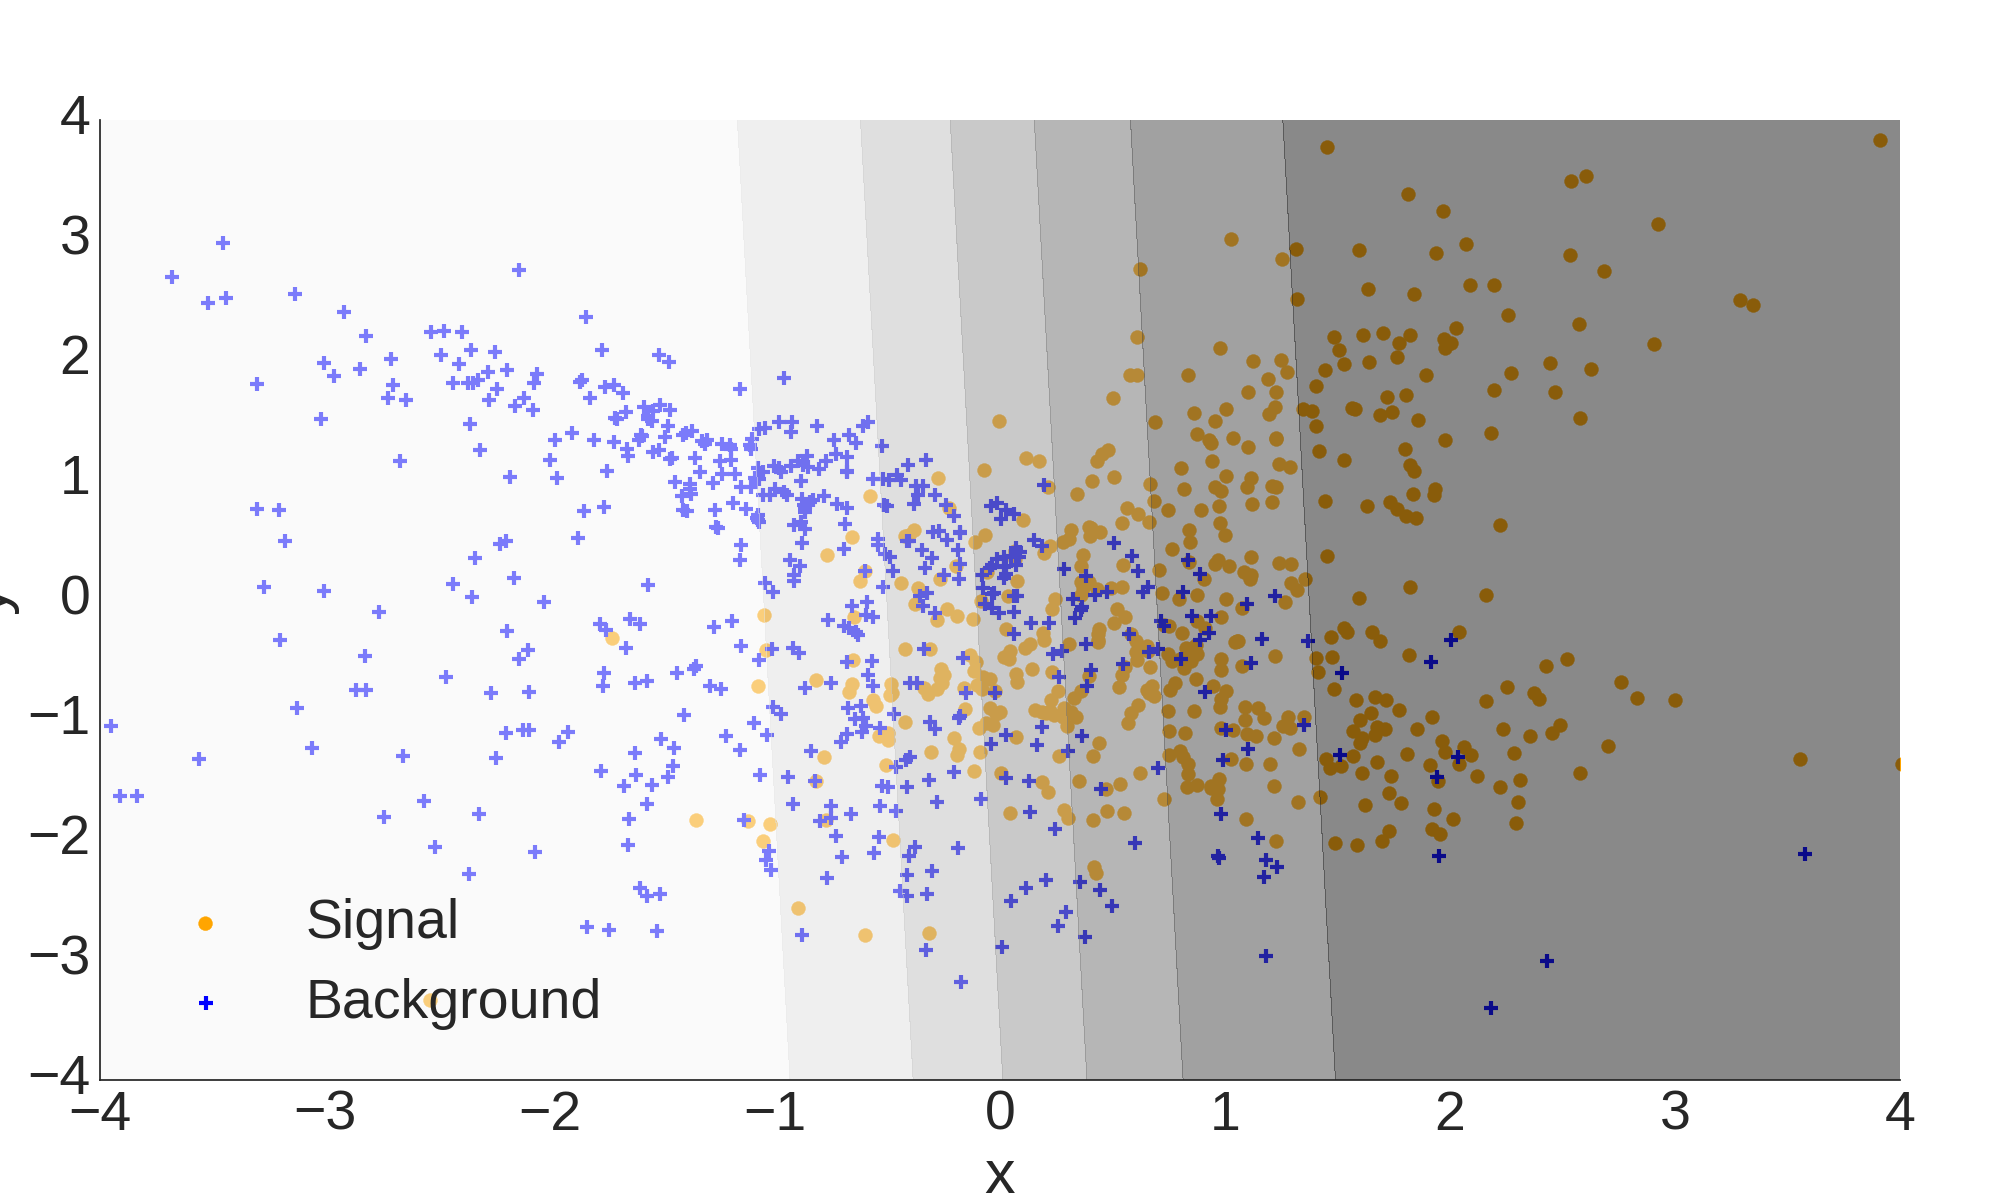
\includegraphics[width=0.6\textwidth]{lda_classifier.png}};
        \end{tikzpicture}
    \end{center}
\end{frame}

\begin{frame}
    \frametitle{Quadratic Discriminant Analysis}
    \begin{center}
		\begin{itemize}
            \item Assumes conditional PDFs are normally distributed
            \item Requires only means $\mu_y$ and covariances $\Sigma_y$ of sample
            \item Separating hyperplane is quadratic
		\end{itemize}


        \vspace{-1em}
        \begin{align*}
            f(\vec{x}) &= \frac{\sqrt{2 \pi | \Sigma_{y=0} |} \exp\left( - \frac{1}{2} \left(x - \mu_{y=1}\right)^T \Sigma^{-1}_{y=1} \left(x - \mu_{y=1}\right)  \right) }{ \sqrt{2 \pi | \Sigma_{y=1} |}  \exp\left( - \frac{1}{2} \left(x - \mu_{y=0}\right)^T \Sigma^{-1}_{y=0} \left(x - \mu_{y=0}\right)  \right)  }
        \end{align*}


        \vspace{-1.5em}
        \begin{tikzpicture}
            \node[anchor=south west,inner sep=0] (image) at (0,0) {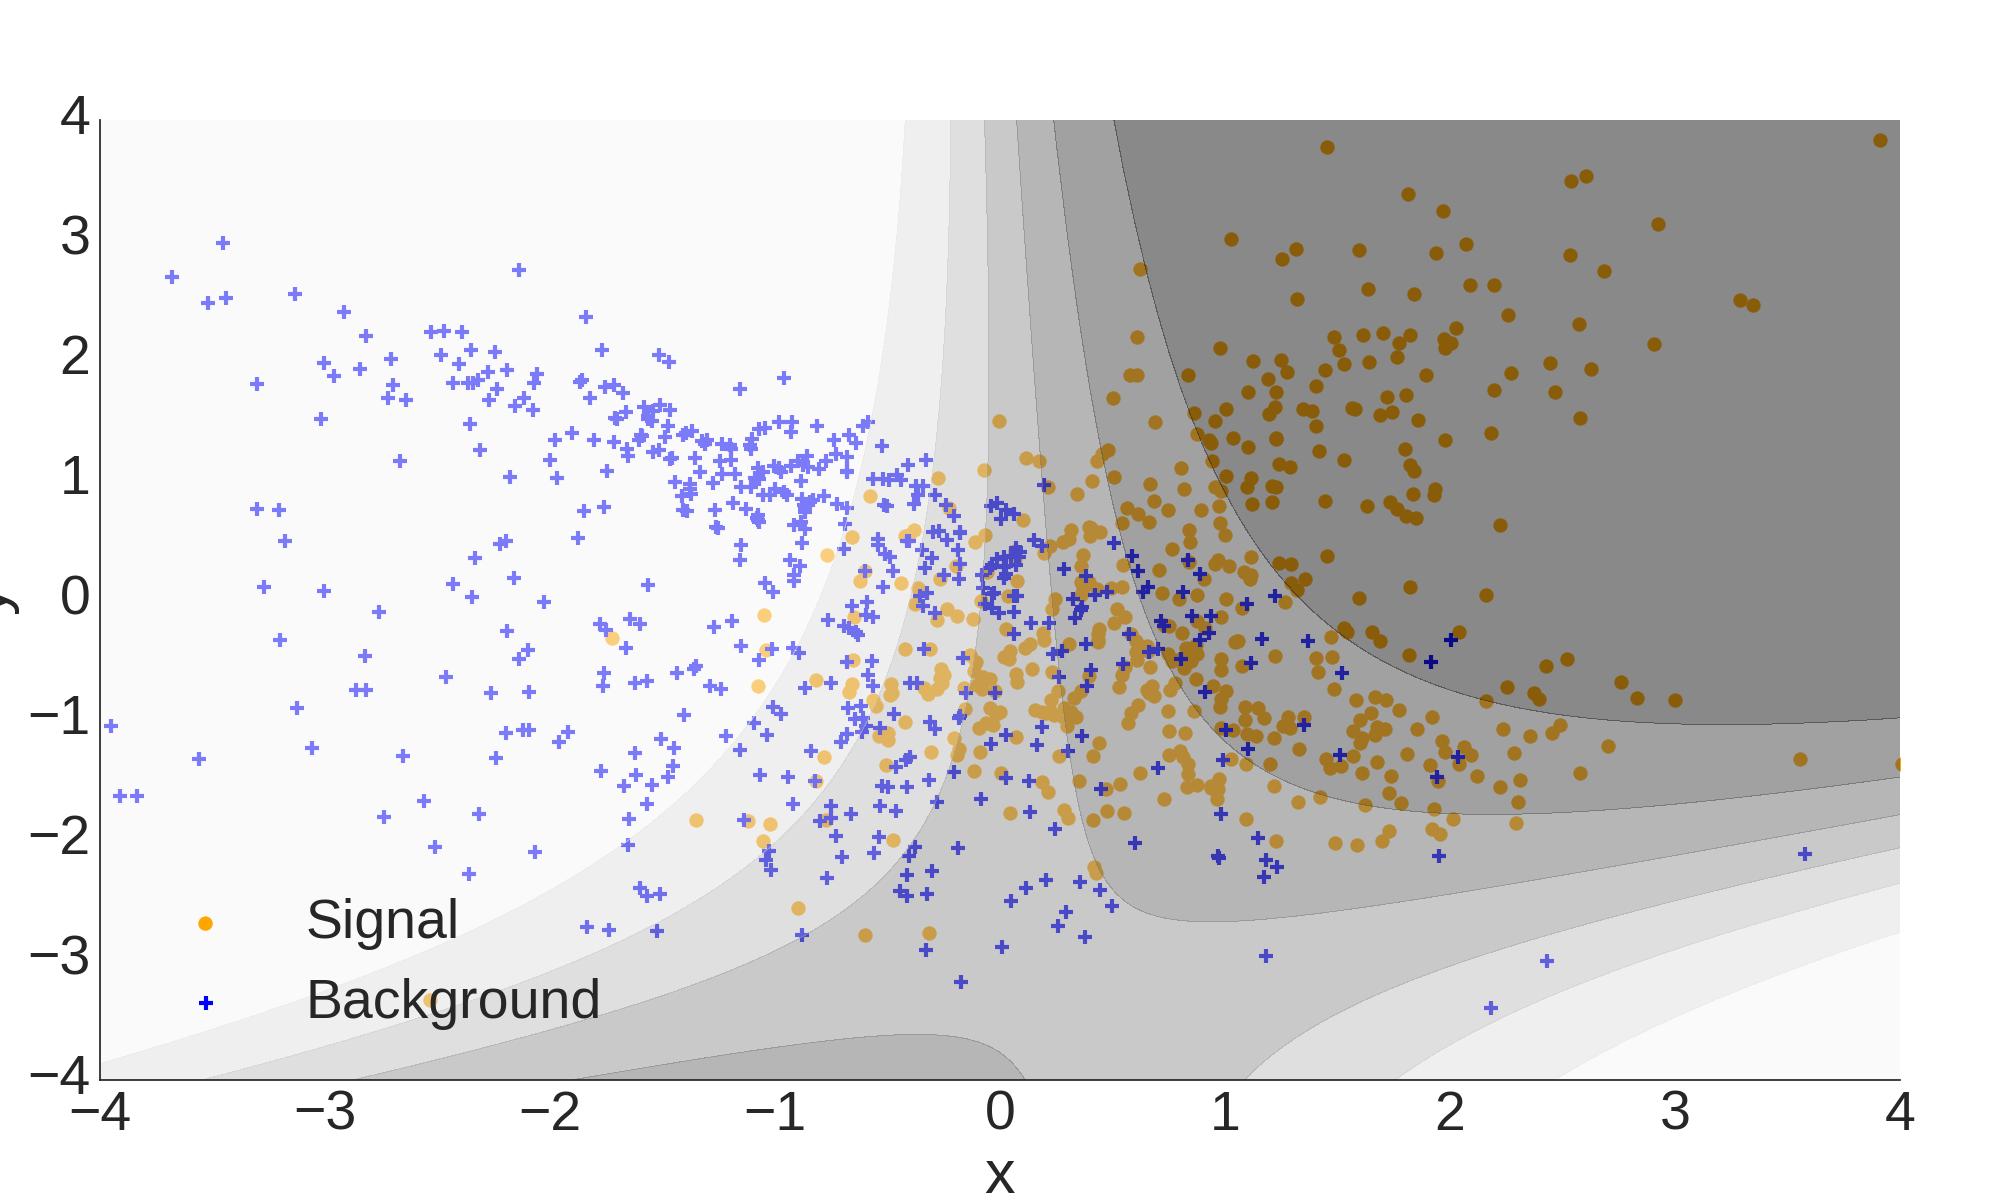
\includegraphics[width=0.6\textwidth]{qda_classifier.png}};
        \end{tikzpicture}
    \end{center}
\end{frame}

\begin{frame}
    \frametitle{Example Classifier Quality}
    \begin{center}
        \begin{tikzpicture}
            \node[anchor=south west,inner sep=0] (image) at (0,0) {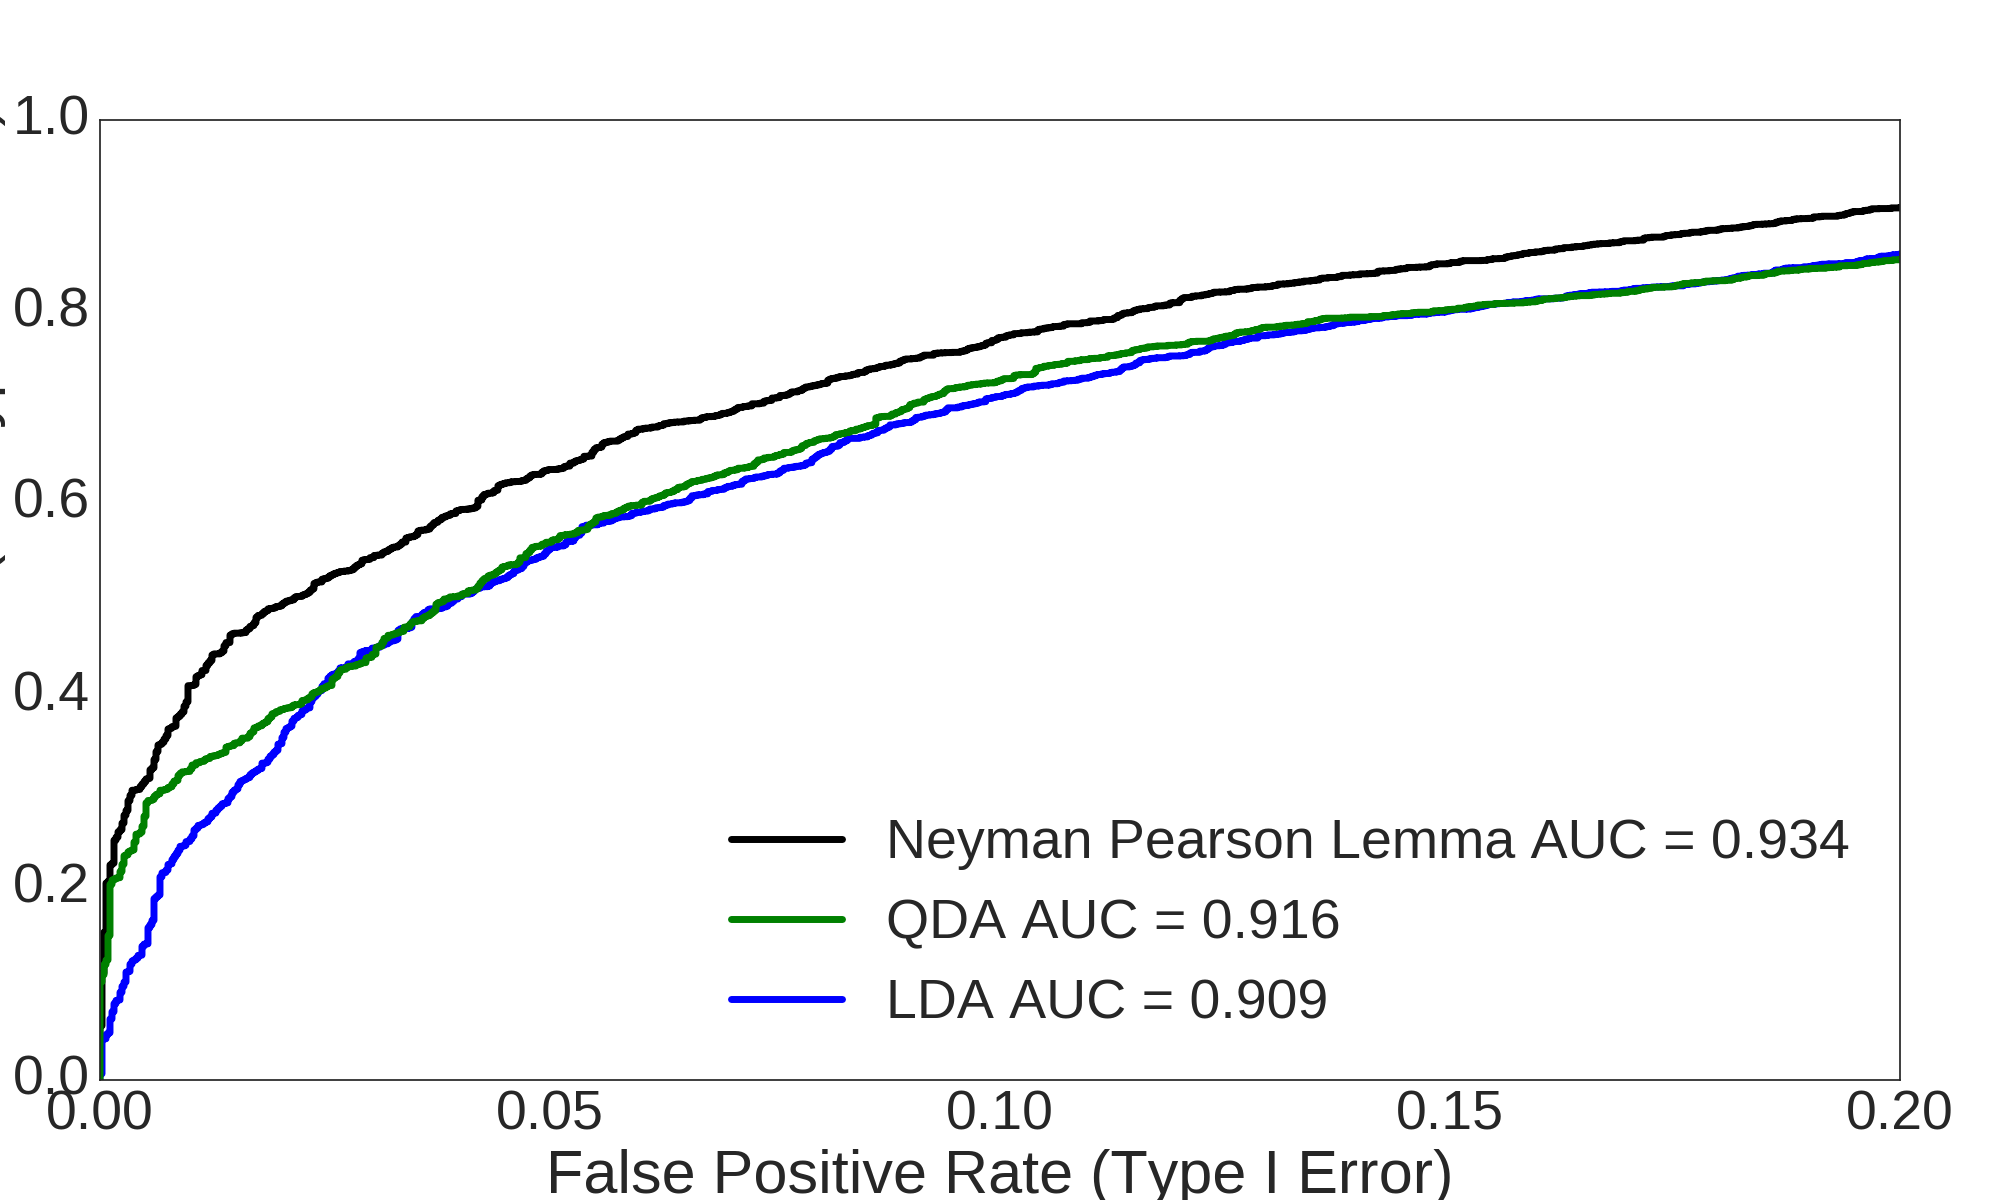
\includegraphics[width=\textwidth]{lda_qda_roc.png}};
        \end{tikzpicture}
    \end{center}
\end{frame}
